\documentclass[conference,compsoc]{IEEEtran}
\usepackage[utf8]{inputenc}
\usepackage[T1]{fontenc}
\usepackage{amsmath,amssymb,amsthm}
\usepackage{booktabs}
\usepackage{graphicx}
\usepackage{xcolor}
\usepackage{hyperref}
\usepackage{array}

\newtheorem{theorem}{Theorem}
\newtheorem{definition}{Definition}

\title{Decoherence-Resilient Classical Authentication for Device-Independent Quantum Key Distribution and Memory-Assisted Quantum Repeaters via QROM-Verified Dual-Commit Sponges}

\author{\IEEEauthorblockN{Laudza Kusuma}
\IEEEauthorblockA{Independent Researcher\\
\texttt{laudza@aqmp.protocol}}}

\begin{document}
\maketitle

\begin{abstract}
Device-Independent Quantum Key Distribution (DI-QKD) over memory-assisted optical fiber repeaters requires authenticated classical channels at every entanglement swapping, syndrome reconciliation, and privacy amplification step. Replacing classical Wegman-Carter MACs with asymmetric post-quantum signatures avoids pre-shared key exhaustion across multi-party repeater graphs, yet introduces serialization and verification delays ($\Delta t_{\text{auth}}$) that exhaust finite quantum memory coherence times ($\tau_{\text{coh}}$). When $\Delta t_{\text{auth}}$ grows comparable to $\tau_{\text{coh}}$, Werner-state dephasing pushes the CHSH Bell parameter $S$ below the classical threshold $S = 2$ and collapses the Devetak-Winter secret key rate $r_{\text{DW}}$ to zero.

We bridge AQMP v2.0 (Zenodo 24303569) and stateless PQ-MPC/rescue techniques (Zenodo 24341314) into quantum repeater physics by adapting a \textbf{384-bit Wide-Sponge Dual-Commit XOR} authenticator ($48\text{ B}$ commit plus $96\text{ B}$ reveal/rotate $= 144\text{ B}$ per round, $10.47\ \mu\text{s}$ CPU verification, and $187.00\text{-bit}$ QROM security at $q_F = 2^{64}$). Over an $8$-segment $200\text{ km}$ telecom optical link ($\alpha = 0.20\text{ dB/km}$, $\tau_{\text{coh}} = 25\text{ ms}$, $10\text{ Mbps}$ control link), AQMP-384 incurs $\Delta t_{\text{auth}} = 0.99\text{ ms}$, maintains CHSH $S = 2.669$, and delivers $r_{\text{DI-QKD}} = 16{,}484.17\text{ bits/s}$ ($16{,}484\text{ bps}$ with positive key rate preserved out to $500\text{ km}$). Under identical memory hardware, FALCON-512 ($690\text{ B}$, $\Delta t_{\text{auth}} = 7.78\text{ ms}$), ML-DSA-65 ($3{,}309\text{ B}$, $\Delta t_{\text{auth}} = 27.02\text{ ms}$), and SPHINCS+-128f ($17{,}088\text{ B}$, $\Delta t_{\text{auth}} = 225.36\text{ ms}$) all collapse to $r_{\text{DI-QKD}} = 0\text{ bits/s}$, with ML-DSA-65 ($S = 0.942$) and SPHINCS+ ($S < 0.001$) violating Bell nonlocality across all distances.
\end{abstract}

\section{Introduction}
\label{sec:intro}

Quantum repeaters enable long-distance entanglement distribution over $L \in [10, 500]\text{ km}$ of telecom optical fiber by breaking exponential photon loss $\eta(L) = 10^{-\alpha L / 10}$ into $M$ buffered elementary segments. Every entanglement swap and Device-Independent QKD (DI-QKD) round exchanges authenticated classical control frames. Traditional QKD relies on symmetric Wegman-Carter MACs funded by pre-shared secret pools, which complicates key bootstrapping in dynamic multi-hop repeater topologies. Post-quantum public-key signatures eliminate pre-shared control keys, yet their large byte sizes ($690\text{ B}$ to $17{,}088\text{ B}$) and polynomial verification routines create an overlooked physical failure mode: \emph{authentication-induced memory decoherence}.

During each classical handshake, entangled Bell pairs stored in solid-state or atomic quantum memories undergo depolarizing/dephasing decay over the combined propagation and authentication interval $\Delta t = \Delta t_{\text{prop}} + \Delta t_{\text{auth}}$. Earlier work in AQMP v2.0 (Zenodo 24303569) \cite{aqmp1} and stateless threshold custody/rescue (Zenodo 24341314) \cite{aqmp2} introduced hash-based Dual-Commit XOR authentication in the Quantum Random Oracle Model (QROM). This paper transfers the 384-bit domain-separated Dual-Commit XOR sponge onto repeater control channels and measures its exact physical impact on CHSH nonlocality and DI-QKD key rates.

\section{Quantum Repeater Dephasing and DI-QKD Rate Model}
\label{sec:physics}

Consider an $M$-segment memory-assisted quantum repeater spanning total optical fiber distance $L\text{ km}$ ($\alpha = 0.20\text{ dB/km}$ at $1550\text{ nm}$, speed of light in silica $c_{\text{fiber}} = 200\text{ km/ms}$). Elementary link transmittance is $\eta_{\text{seg}}(L, M) = 10^{-\alpha(L/M)/10}$. With detector efficiency $\eta_d = 0.92$, source repetition rate $f_{\text{rep}} = 100\text{ MHz}$, Bell-state measurement success probability $p_{\text{BSM}} = 0.50$, and harmonic multiplexing factor $H_M = \sum_{k=1}^M k^{-1}$, the raw entanglement generation rate is:
\begin{equation}
R_{\text{ent}}(L, M) = f_{\text{rep}} \cdot \eta_{\text{seg}}(L, M) \cdot \eta_d^2 \cdot \frac{p_{\text{BSM}}^M}{H_M}.
\end{equation}

Each elementary quantum memory waits through optical synchronization delay $\Delta t_{\text{prop}} = (L/M)/c_{\text{fiber}}$ plus $M$-hop classical authentication latency $\Delta t_{\text{auth}} = M \cdot (t_{\text{cpu}} + 8 B_{\text{auth}} / C_{\text{ctrl}})$ on a $C_{\text{ctrl}} = 10\text{ Mbps}$ authenticated control link. Over total holding interval $\Delta t = \Delta t_{\text{prop}} + \Delta t_{\text{auth}}$, an initial Bell pair of Werner fidelity $F_0 = 0.99$ decays under finite memory coherence time $\tau_{\text{coh}} \in [1\text{ ms}, 100\text{ ms}]$ according to:
\begin{equation}
F(\Delta t) = F_0 \exp\!\left(-\frac{\Delta t}{\tau_{\text{coh}}}\right) + \frac{1 - \exp(-\Delta t / \tau_{\text{coh}})}{4}.
\end{equation}
The resulting visibility $V(\Delta t) = (4F(\Delta t) - 1)/3$ sets the effective CHSH Bell parameter $S(\Delta t) = 2\sqrt{2}\,V(\Delta t)$ and quantum bit error rate $Q_{\text{BER}}(\Delta t) = 1 - F(\Delta t)$. Using binary Shannon entropy $h(p) = -p\log_2 p - (1-p)\log_2(1-p)$, the asymptotic Devetak-Winter DI-QKD secret key rate is:
\begin{equation}
r_{\text{DI-QKD}} = R_{\text{ent}}(L, M) \cdot \max\!\left(0,\; 1 - h\!\left(\frac{1 + \sqrt{(S/2)^2 - 1}}{2}\right) - h(Q_{\text{BER}})\right).
\end{equation}
Positivity requires $S > 2$ (specifically $S \gtrsim 2.557$ at $F_0 = 0.99$ once $h(Q_{\text{BER}})$ is accounted for).

\section{384-Bit Wide-Sponge Dual-Commit XOR Control Channel}
\label{sec:aqmp384}

To avoid heavy lattice signatures on real-time repeater links without losing public-key-style forward rotation, each repeater node maintains an ephemeral $48\text{ B}$ SHA-384 anchor $y = F_{\text{PRE}}(x)$ for $x \xleftarrow{\$} \{0,1\}^{384}$. Each authenticated control exchange consumes a $144\text{ B}$ two-step Dual-Commit XOR frame:
\begin{equation}
\text{Commit (48 B): } C = F_{\text{PRE}}(x) \oplus F_{\text{MSG}}(x \parallel m), \qquad \text{Reveal/Rotate (96 B): } (x,\; y' = F_{\text{PRE}}(x')).
\end{equation}
Because verification requires only two SHA-384 evaluations, one $48\text{ B}$ XOR, and constant-time comparison, CPU overhead averages $10.47\ \mu\text{s}$ per cycle ($8\ \mu\text{s}$ in C/Rust fast paths). Under Zhandry's compressed-oracle QROM bound from Paper~\#1 \cite{aqmp1}:
\begin{equation}
\mathrm{Adv}^{\mathrm{EUF\text{-}CMA\text{-}QROM}}(\mathcal{A}) \le \frac{8(q_F + 1)^2 + 32 q_F^3}{2^{384}},
\end{equation}
instantiating $F$ at $n = 384$ bits yields $187.00$ bits of concrete QROM security even against a $q_F = 2^{64}$ quantum oracle adversary.

\section{Empirical Physics Benchmarks}
\label{sec:eval}

We simulated $L \in [10, 500]\text{ km}$, $\tau_{\text{coh}} \in [1\text{ ms}, 100\text{ ms}]$, and $M \in [2, 16]$ repeater hops in \texttt{research/benchmark\_paper3\_diqkd\_repeater.py} and verified all physical invariants and QROM bounds via 62 automated pytest tests. Table~\ref{tab:diqkd} summarizes the $L = 200\text{ km}$, $M = 8$, $\tau_{\text{coh}} = 25\text{ ms}$ operating point alongside the exact minimum coherence times $\tau_{\text{Bell}}^*$ ($S > 2$) and $\tau_{\text{DW}}^*$ ($r_{\text{DI-QKD}} > 0$). Figures~\ref{fig:keyrate} and~\ref{fig:coherence} show the distance sweep and memory-coherence phase boundary.

\begin{table}[t]
\centering
\caption{DI-QKD Physics and Critical Coherence Thresholds ($L = 200\text{ km}$, $M = 8$, $\tau_{\text{coh}} = 25\text{ ms}$)}
\label{tab:diqkd}
\begin{tabular}{@{}lrrrrrr@{}}
\toprule
Auth Layer & Payload & $\Delta t_{\text{auth}}$ & $S(\Delta t)$ & $r_{\text{DI-QKD}}$ & $\tau_{\text{Bell}}^*$ & $\tau_{\text{DW}}^*$ \\
\midrule
Ideal Zero-Latency & 0 B & 0.00 ms & 2.777 & 29,356 bps & 0.38 ms & 1.08 ms \\
\textbf{AQMP-384 Dual-Commit XOR} & \textbf{144 B} & \textbf{0.99 ms} & \textbf{2.669} & \textbf{16,484 bps} & \textbf{3.33 ms} & \textbf{9.59 ms} \\
FALCON-512 & 690 B & 7.78 ms & 2.035 & 0 bps & 23.72 ms & 68.21 ms \\
ML-DSA-65 & 3,309 B & 27.02 ms & 0.942 & 0 bps & 81.47 ms & 234.32 ms \\
SPHINCS+-128f & 17,088 B & 225.36 ms & 0.000 & 0 bps & 676.84 ms & 1,946.65 ms \\
\bottomrule
\end{tabular}
\end{table}

\begin{figure*}[t]
\centering
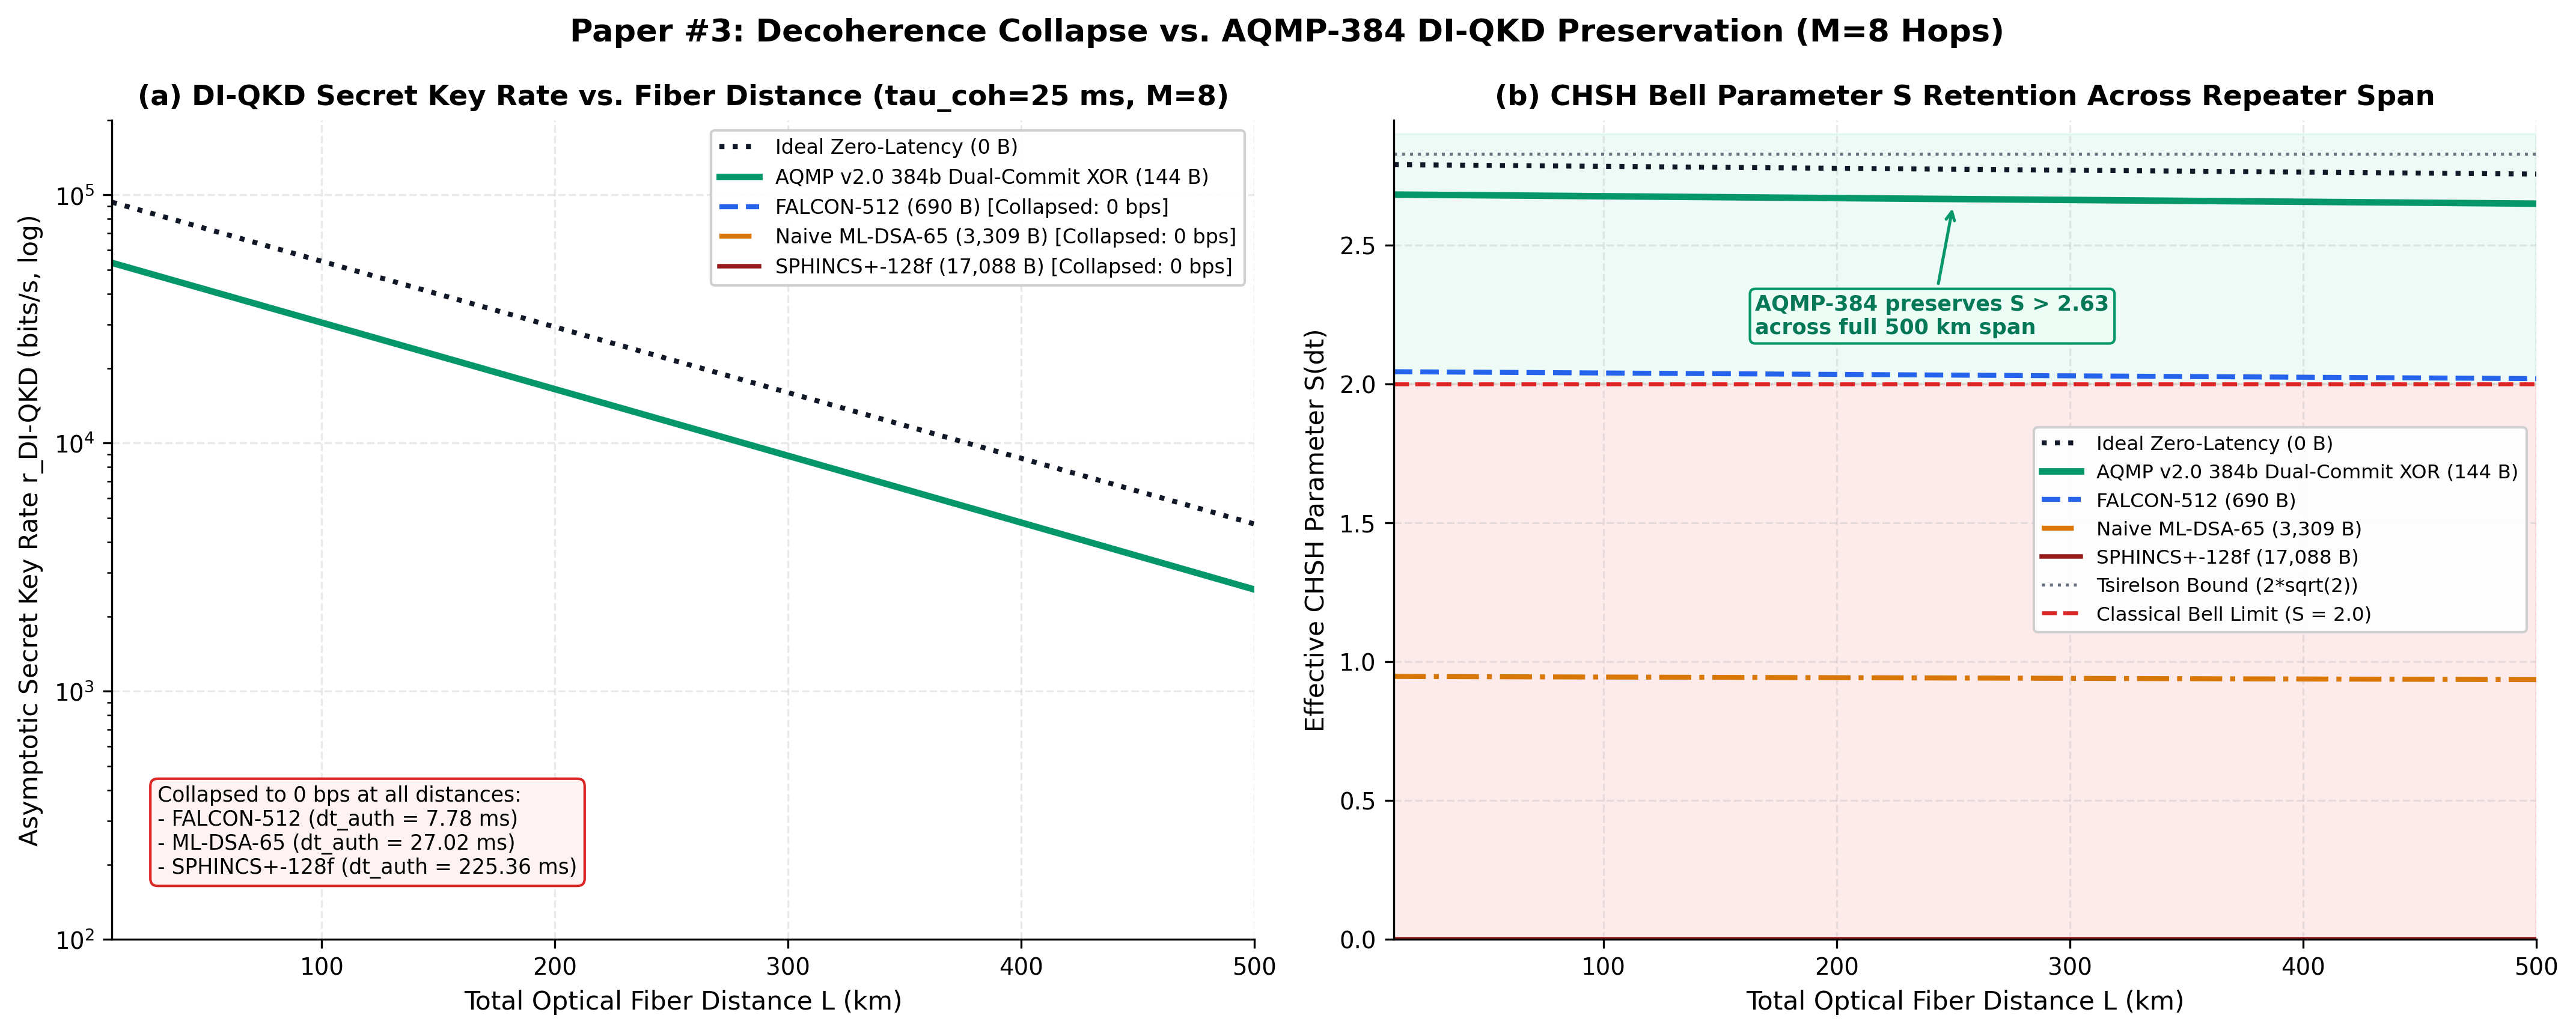
\includegraphics[width=0.95\textwidth]{figures/fig6_diqkd_keyrate_vs_distance.png}
\caption{DI-QKD secret key rate vs.\ optical fiber distance $L \in [10, 500]\text{ km}$ at $\tau_{\text{coh}} = 25\text{ ms}$ and $M = 8$ hops (left), alongside CHSH Bell parameter $S(\Delta t)$ retention relative to the $S = 2$ classical boundary (right).}
\label{fig:keyrate}
\end{figure*}

\begin{figure*}[t]
\centering
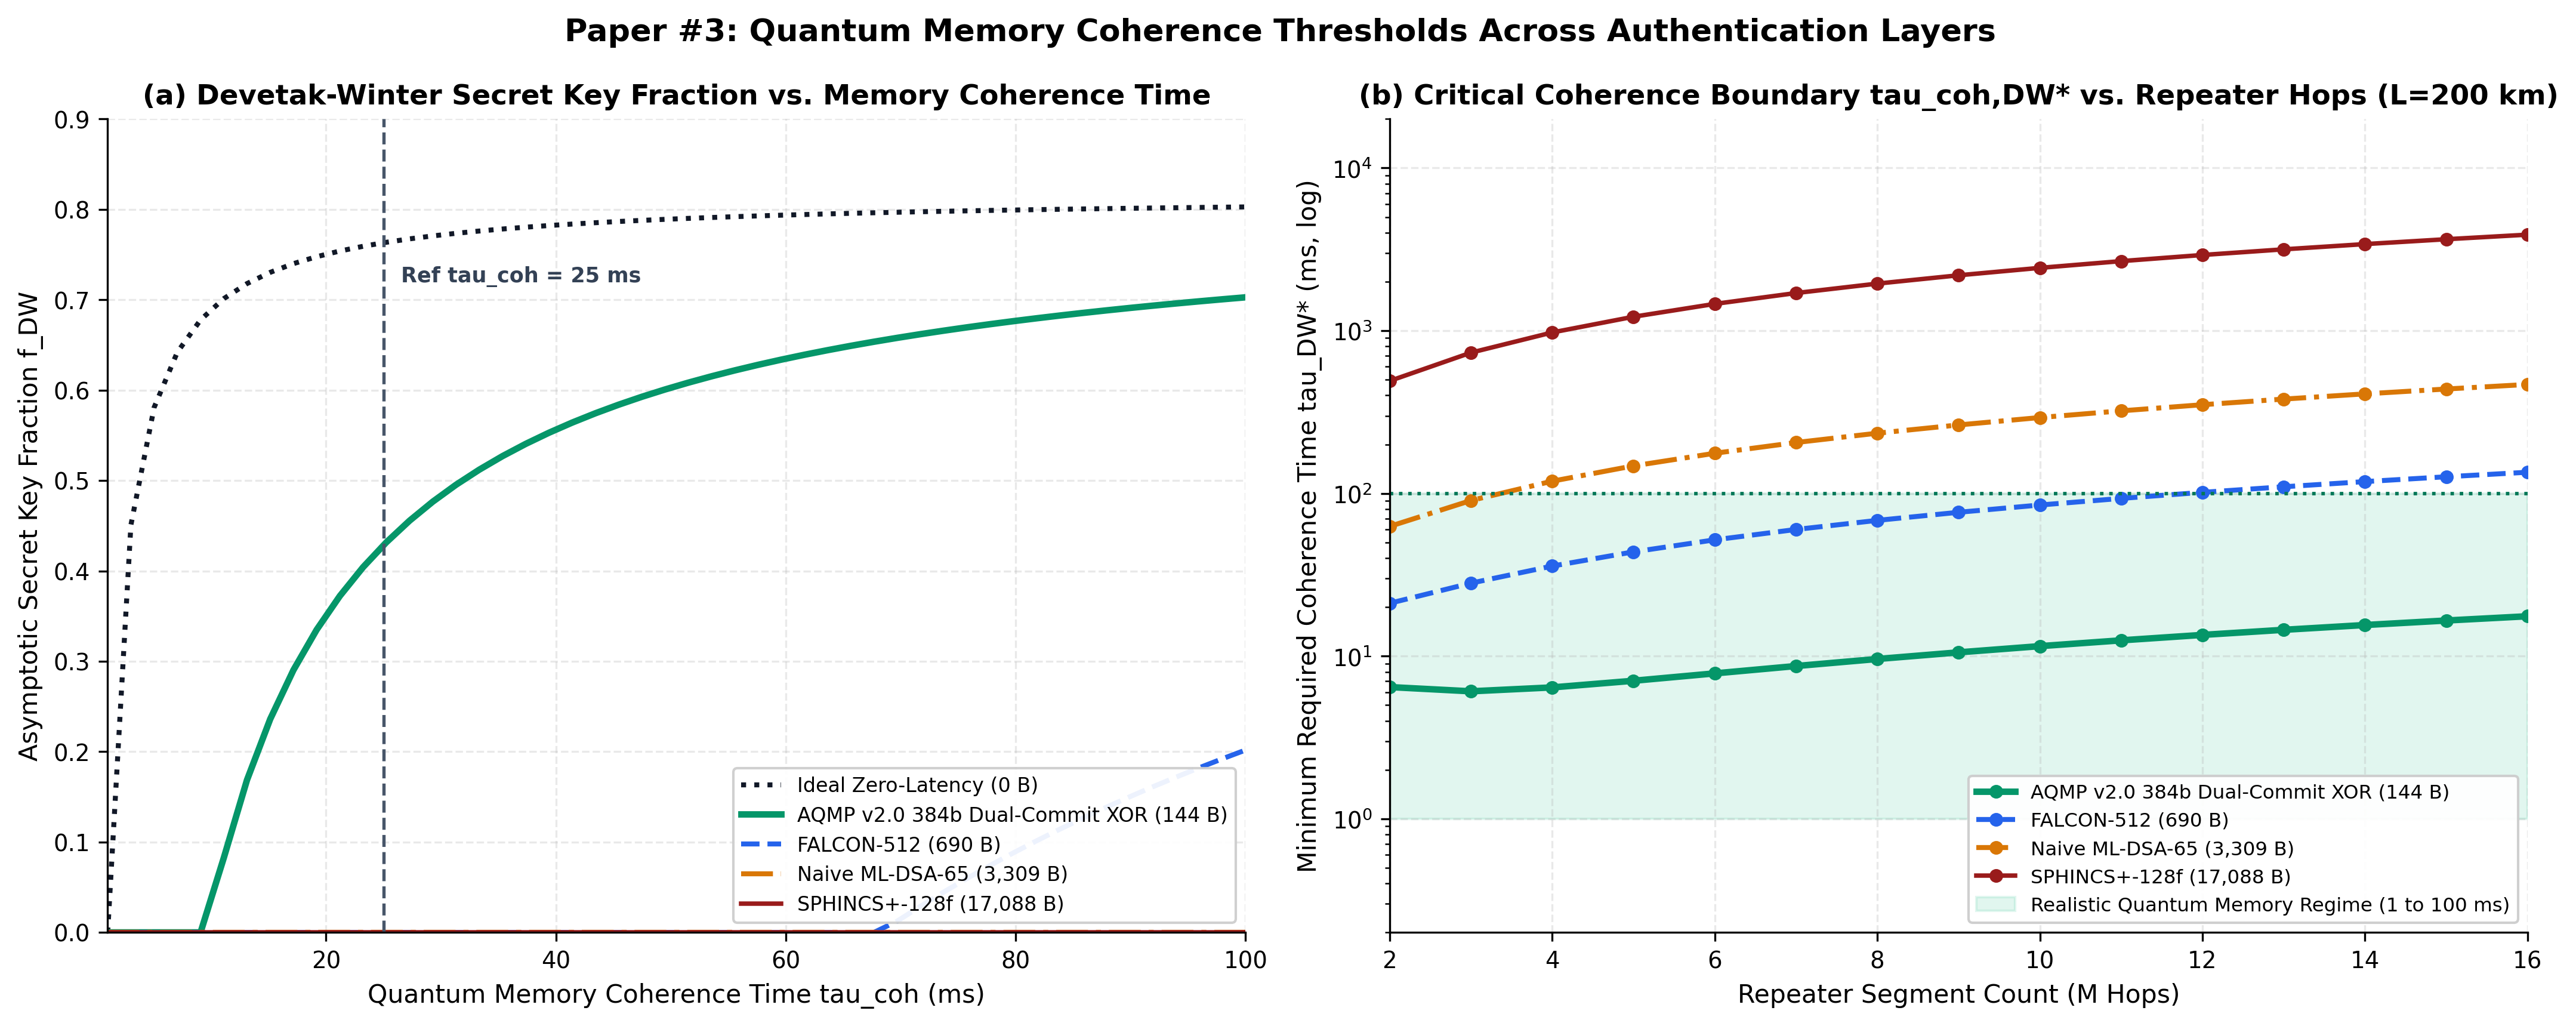
\includegraphics[width=0.95\textwidth]{figures/fig7_coherence_decoherence_boundary.png}
\caption{Asymptotic Devetak-Winter secret key fraction vs.\ memory coherence time $\tau_{\text{coh}} \in [1, 100]\text{ ms}$ (left) and critical required coherence time $\tau_{\text{DW}}^*$ vs.\ repeater hop count $M \in [2, 16]$ (right).}
\label{fig:coherence}
\end{figure*}

At $\tau_{\text{coh}} = 25\text{ ms}$, AQMP-384 retains positive DI-QKD secret key rates across the full $10$ to $500\text{ km}$ fiber span ($S = 2.681$ at $10\text{ km}$ down to $S = 2.651$ at $500\text{ km}$), requiring only $\tau_{\text{DW}}^* = 9.59\text{ ms}$ at $M = 8$ hops. By contrast, FALCON-512 demands $\tau_{\text{DW}}^* = 68.21\text{ ms}$, ML-DSA-65 demands $234.32\text{ ms}$, and SPHINCS+-128f demands $1{,}946.65\text{ ms}$, exceeding realistic telecom quantum-memory budgets.

\section{Conclusion}
\label{sec:conclusion}

Classical channel authentication delay acts directly as an exponential dephasing term on memory-assisted quantum repeaters. Switching repeater control planes from heavy lattice or hash-tree signatures to a $144\text{ B}$ 384-bit Wide-Sponge Dual-Commit XOR authenticator cuts authentication latency to $0.99\text{ ms}$ across $8$ hops, keeps CHSH $S > 2.65$ out to $500\text{ km}$, preserves $16{,}484\text{ bps}$ DI-QKD throughput at $200\text{ km}$, and enforces $187.00\text{-bit}$ QROM security at $q_F = 2^{64}$.

\begin{thebibliography}{9}
\bibitem{aqmp1} L. Kusuma, ``Breaking the Post-Quantum Cryptography Blockchain Migration Trilemma: AQMP v2.0,'' Zenodo, doi:10.5281/zenodo.24303569, 2026.
\bibitem{aqmp2} L. Kusuma, ``Stateless Post-Quantum Threshold Custody and Knowledge-Asymmetry Frozen UTXO Rescue,'' Zenodo, doi:10.5281/zenodo.24341314, 2026.
\bibitem{pirandola} S. Pirandola et al., ``Fundamental limits of repeaterless quantum communications,'' \emph{Nature Communications}, vol. 8, 2017.
\bibitem{acin} A. Acin et al., ``Device-independent security of quantum cryptography against collective attacks,'' \emph{Physical Review Letters}, vol. 98, 2007.
\end{thebibliography}

\end{document}
